%Ideally, we could choose $N$, $D$, and $B$ based on time or compute
%constraints, and be confident that the resulting models would be
%well-tuned.

%Good HPs enable good training, and also good scaling laws.

%%
%Before we could reliably measure $B$ scaling, we found AdamW HPs to be
%suboptimal under $\mup$ as $B$, $D$ varied.
%%
%This led to our study of optimal HPs, culminating in the $\tepoch$
%scaling law.

\subsection{Background: $\mup$, AdamW, and $\tepochwang$}

\paragraph{$\mup$}\label{sec:mup}
%
$\mup$ is increasingly used in LLM
training~\citep{dey2023cerebras,dey2023btlm3b8k,sengupta2023jais,shen2024power,hu2024minicpm,abdin2024phi}.
%
With $\mup$, base HPs are tuned on a \emph{proxy} model and then
transferred to wider~\citep{yang2022mup} and
deeper~\citep{dey2025dont} models.
%with scaling factors for learning rate, initial weight variance, and
%other HPs dependent on the relative width of the proxy and target
%models.
Given the width of the proxy model, $d_p$, and target, $d_t$, $\mup$
prescribes scaling factors to apply to the LR, initial weight
variance, and other base HPs.
%
In particular, the optimal base LR, $\hatetaopt$ is scaled down to
$\etaopt = (\nicefrac{d_p}{d_t})\hatetaopt$.
%
%$\mup$ also uses scaling to stabilize embeddings, layer norms, and
%self-attention in transformers.
%
%Might reference \citet{dey2023cerebras} for how they adjust $B$ for
%MUP\@.  Note they don't say how to estimate $\cbs$.

While $\mup$ enables the same base LR to be used across different $N$,
$\hatetaopt$ has empirically been found to \emph{vary with
$B$}~\citep{yang2022mup,lingle2024large,noci2024learning,shen2024power}.
%
Moreover, recent work has also observed $\hatetaopt$ \emph{decreasing
in $D$}, leading to proposals for scaling $\hatetaopt$ as a
(decreasing) power law in $D$~\citep{shen2024power,bjorck2024scaling}.
%
%In our experiments with AdamW, when $B$ and $D$ change, we
%consistently find it more effective to adjust $\lambda$ rather than
%$\eta$.

\paragraph{The EMA view of AdamW}\label{sec:ema}

Rather than adjusting $\eta$ as $D$ scales, \citet{wang2024how}
proposed that, if using the AdamW
optimizer~\citep{loshchilov2017decoupled} with $\mup$, then the weight
decay, $\lambda$, should instead be adjusted.
%
To see this, note an AdamW update at each step, $t$, can be expressed
in terms of $\eta \lambda$ as:
\begin{equation}\label{eq:adamw}
\theta_t = (1 - \eta\lambda)\theta_{t-1} - \eta \frac{\hat{m}_t}{\sqrt{\hat{v}_t} + \epsilon}
\end{equation}
%
Here, $\eta$ is the $\mup$-adjusted LR, and $\hat{m}_t$ and
$\hat{v}_t$ are (bias-corrected) exponentially-weighted moving
averages (EMAs) of gradients and squared
gradients~\citep{kingma2014adam}. \citet{wang2024how} observed AdamW's
parameters, $\theta_t$, can \emph{also} be viewed as an EMA---of
weight \emph{updates}.  Specifically, the standard EMA form \mbox{$y_t
  = (1 - \alpha)y_{t-1} + \alpha x_t$} matches AdamW when
%\begin{equation}\label{eq:adamwema}
\mbox{$y_t=\theta_t$}, \mbox{$\alpha=\eta\lambda$}, and
\mbox{$x_t=-\frac{1}{\lambda}\frac{\hat{m}_t}{\sqrt{\hat{v}_t} + \epsilon}$}.
%\end{equation}
The quantity $\nicefrac{1}{\alpha} = \nicefrac{1}{\eta\lambda}$
provides a measure of the number of iterations (i.e., steps) over
which updates are averaged;
\citet{wang2024how} denote it as $\titer$.
%
They show that if the timescale is measured in \emph{epochs} as
$\tepochwang = {\titer}/{M}$, where $M$ is iterations-per-epoch, then
the optimal $\tepochwang$ remains stable when $N$ or $D$ scale (on
image tasks).  I.e., if $M$ scales up, $\lambda$ should be
scaled \emph{down} to maintain constant $\tepochwang$.
%i.e., $M$ increases, $\lambda$ should be scaled down accordingly.
%
%they did not experiment with compute-optimal LLMs, but mainly image
%recognition datasets).
%
%%
%they recommend keeping
%$\tepochwang$ constant via a corresponding adjustment to
%$\lambda$.
%
%We expand on this approach below and show how to successfully use it
%when both $D$ \emph{and} $B$ vary.

\subsection{Methods: The AdamW timescale for LLMs, $\tepoch$, and its scaling}\label{sec:tema_methods}

%\paragraph{$\lambda$ scales with $B$}

Since LLM pre-training only uses one ``epoch'' of data, we normalize
the timescale as $\tepoch = {\titer}/{S}$, where $S$ is the total
number of optimization steps.\footnote{Because it depends on $\eta$,
timescale $\tepoch$ \emph{varies} during LR decay. Here we compute
$\tepoch$ at peak LR\@. Notably, if two training runs share the same
LR schedule (shape) and $\tepoch$ (at peak LR), their final AdamW
timescale (EMA contributions over the \emph{data}) will match---even
if $B$ differs. \cref{sec:ema_lr} provides further details.}
%
Moreover, since $S$=${D}/{B}$,
%then $\tepoch = \titer(\nicefrac{B}{D})$, i.e.,
%Given $\titer = \nicefrac{1}{\eta\lambda}$,
\begin{equation}\label{eq:tepoch}
  \tepoch = \frac{B}{\eta\lambda D}
\end{equation}

$\tepoch$ reflects the fraction of past iterations to include in the
final weights.
%
While \citet{wang2024how} did not vary $B$, their work suggests this
fraction should remain constant as $B$ scales.
%
We hypothesize that when moving from compute-efficient to overtrained
LLMs, updates can be integrated over a smaller fraction of the data;
specifically, that $\tepochopt$ decreases as a power law in $\tpp :=
\nicefrac{D}{N}$:
\begin{equation}\label{eq:tepoch_scaling}
  \tepochopt(\tpp) = \ctepoch \cdot \tpp^{\mtepoch}
\end{equation}
where $\ctepoch$ and $\mtepoch$ are parameters to be fit.
%
%In the following results, we demonstrate excellent fits to
%\cref{eq:tepoch_scaling} on our experimental data.
%
Appendix \cref{alg:tepoch_fitting} summarizes the fitting procedure.
%
%Note we are collecting $\tepoch$ here for runs where $B < \cbs$.
%
Taking the $\mup$-adjusted $\eta$ as our LR, $\lambdaopt$ can be
computed from \cref{eq:tepoch,eq:tepoch_scaling}:
\begin{equation}\label{eq:lambdaopt}
   \lambdaopt = \frac{B}{\eta \cdot D \cdot \tepochopt(\tpp)}
              = \frac{B \cdot \tpp^{-\mtepoch}}{\ctepoch \cdot \eta \cdot D}
\end{equation}

\subsection{Experimental details}\label{sec:lambda_experimental}

We use a GPT2-like LLM~\citep{radford2019gpt2}, with ALiBi
embeddings~\citep{press2022alibi} and SwiGLU~\citep{shazeer2020glu}.
%with the GPT-2 vocabulary (size 50257), and a context length of 2048
%tokens.
%
We train on SlimPajama~\citep{cerebras2023slimpajama} and always
evaluate over a held-out set of 1.1B tokens.
%
We use AdamW and $\mup$, with $\mup$ HPs derived from a smaller proxy
model, and a linear LR schedule, with a 10\% warmup followed by
decay-to-zero~\citep{bergsma2025straight}.
%
\cref{sec:experimental_details} has full experimental details.

\subsection{Results: $\tepoch$ and scaling $\lambda$}\label{sec:tema_results}

\begin{figure}[H]
    \centering
    \begin{minipage}{0.33\textwidth}
        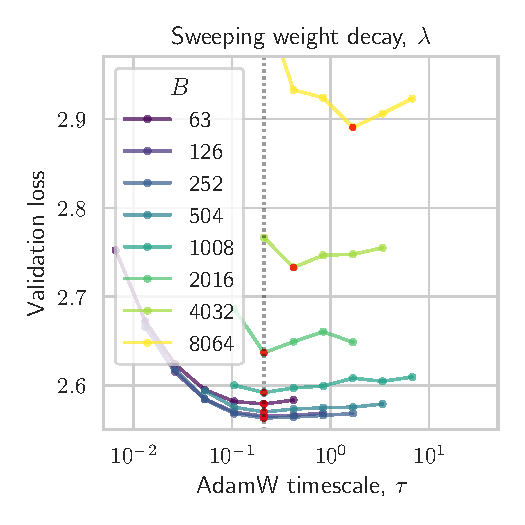
\includegraphics[trim={0.3cm 0.4cm 0.3cm 0.3cm}, clip, width=\linewidth]{pdffigs/loss_data.241005_batchsizes.617M.20tpp.D2Z.tepoch.sweep_wd.pdf}
    \end{minipage}\hfill
    \begin{minipage}{0.33\textwidth}
        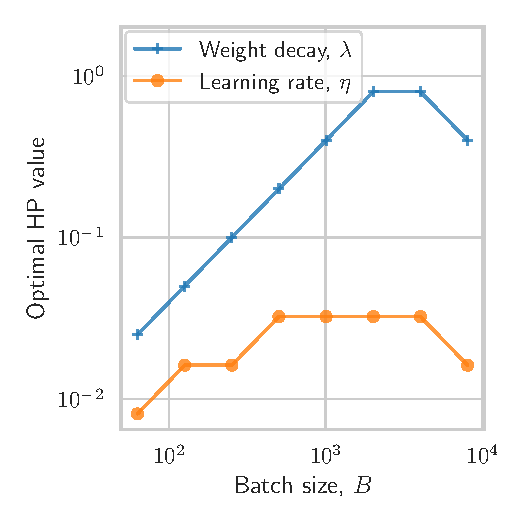
\includegraphics[trim={0.3cm 0.4cm 0.3cm 0.3cm}, clip, width=\linewidth]{pdffigs/loss_data.241005_batchsizes.lr_v_wd.617M.20TPP.pdf}
    \end{minipage}\hfill
    \begin{minipage}{0.33\textwidth}
        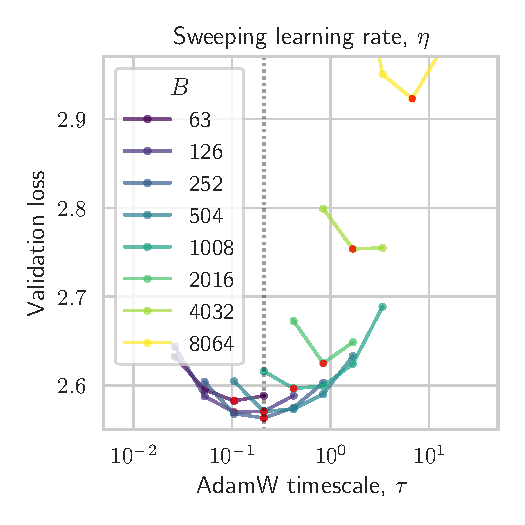
\includegraphics[trim={0.3cm 0.4cm 0.3cm 0.3cm}, clip, width=\linewidth]{pdffigs/loss_data.241005_batchsizes.617M.20tpp.D2Z.tepoch.sweep_lr.pdf}
    \end{minipage}
    \caption{(610M 20TPP): For each $B$, we sweep $\lambda$ and find
      $\tepochopt$ ($\leftfig$). $\tepochopt$ is stable around 0.21
      for $B \in [63, 2016]$, meaning $\lambdaopt$ scales linearly
      with $B$ over this range ($\middlefig$).  When sweeping $\eta$
      ($\rightfig$), the lower boundary over all curves is a bowl with
      a minimum at 0.21; the smallest $B$ settings have $\tepochopt$
      within 2$\times$ of this value, but as $B$ increases,
      $\tepochopt$ quickly drifts higher.\label{fig:tepochs}}
\end{figure}


\finding{The optimal $\tepoch$ remains stable as $B$ scales; $\lambdaopt$ scales linearly with $B$
(\cref{fig:tepochs}).}

As $B$ increases and $\lambda$ is tuned, we find that $\tepochopt$
remains roughly constant---i.e., changes in $B$ lead to commensurate
changes in $\lambdaopt$ (\cref{fig:tepochs}, $\middlefig$)---but only
up to a certain point, after which $\tepochopt$ begins to drift. The
drift point corresponds to the critical batch size $\bcrit$, above
which gradient information no longer scales linearly with $B$ and
diminishing returns set in (\cref{sec:bcrit}).%
\footnote{Training with $B > \cbs$ can be viewed as training with less
\emph{effective} data, thus decreasing the TPP, and shifting
$\temaopt$ higher (by our power law) and thus $\lambdaopt$
\emph{lower}.
%
A decrease in the optimal learning rate $\etaopt$ when $B > \cbs$ has
been previously observed~\citep{li2024surge,filatov2024time}.  These
works measure $\etaopt$ at very large batch sizes, e.g., $10\times$ or
$100\times$ $\bcrit$, which was not practical at the scales that we
trained.  Nevertheless, our observation of a similar ``surge''
phenomenon with $\lambdaopt$, occurring in AdamW rather than vanilla
Adam, motivates further study.}

If $\eta$ is tuned instead, $\etaopt$ fails to scale with $B$ up to
$\bcrit$ (\cref{fig:tepochs}, $\middlefig$); we observe instead a
certain maximum $\eta$, above which training becomes unstable; above
this, loss spikes occur from which training does not recover.
Consequently, $\eta$ has less flexibility to scale with $B$; training
stability is more fundamental than timescale.

In general, LLMs typically train faster and utilize hardware better
with larger $B$, but only up to $\bcrit$: beyond this point, much more
data (and compute) is needed to obtain the same loss, without
meaningfully reducing the total number of sequential training steps
(the poor trade-off for $B > \bcrit$ is depicted in
\cref{fig:cbs_panels}). Furthermore, \cref{sec:bcrit} will show that
there is also an \emph{optimal} batch size, $\bopt$, below which loss
is worse and utilization/parallelism suffer (because batches are
small). In practice, LLMs should therefore be trained in the regime
$\bopt \le B \le \bcrit$. Notably, this is precisely the range where
we have shown weight decay to scale predictably with batch size; our
findings therefore support the direct optimization of weight decay in
the most practically relevant training regimes.

\finding{With AdamW, we should adjust $\lambda$, not $\eta$, as $B$ changes.}

\begin{table}
  \centering
  \caption{(610M, 20TPP) Validation losses comparing tuning $\lambda$
    vs.\ $\eta$ across $B$ (data from \cref{fig:tepochs}).\label{tab:lr_v_wd}}
\begin{tabular}{@{}ccr@{}cccccccc@{}}
\toprule
$\hateta$                      & $\lambda$ & $B$$=$                   & 63         & 126        & 252        & 504        & 1008       & 2016       & 4032       & 8064       \\ \midrule
$\maxlr$                       & 0.1       &                    & 2.595          & 2.570          & \textbf{2.563} & 2.573          & 2.599          & 2.649          & 2.755          & 2.923          \\
Tuned                          & 0.1       &                    & 2.583          & 2.570          & \textbf{2.563} & 2.571          & 2.597          & \textbf{2.625} & 2.754          & 2.923          \\
$\maxlr$                       & Tuned     &                    & \textbf{2.579} & \textbf{2.565} & \textbf{2.563} & \textbf{2.570} & \textbf{2.592} & 2.637          & \textbf{2.733} & \textbf{2.891} \\ \bottomrule
\end{tabular}
\end{table}


Since tuning at scale is infeasible, we need a recipe for selecting
HPs in advance.  Unlike $\eta$, optimal $\lambda$ follows a
predictable relationship with $B$ (\cref{fig:tepochs}, $\middlefig$),
making $\lambda$ the more \emph{viable} target for real-world
adjustment.
%
Moreover, since $\eta$ has less flexibility to maintain optimal
timescale, we hypothesize adjusting $\lambda$ could also be
more \emph{effective}.
%
We tested this by comparing either tuning $\eta$ (using a default
$\lambda$=0.1---standard practice in LLM
pre-training~\citep{hoffmann2022empirical,brown2020language,almazrouei2023falcon,alephalpha2024introducing})---or
tuning $\lambda$ (using the $\mup$ proxy-tuned $\eta$).
%
Tuning $\lambda$ was strictly superior in 6 of 8 cases (\cref{tab:lr_v_wd}).
%
%This table also shows the drawbacks of using default HP settings;
%models obtain over 1\% worse error at large and small $B$---which
%drastically affects $\cbs$ estimation.
%
%For $B$=1008, we also swept the full cross-product of $\eta$
%vs.\ $\lambda$ values; we found tuning $\lambda$ alone remains
%optimal.

We also compared adjusting $\lambda$ versus $\eta$ as $D$ changes.
For a 111M 200TPP model, default HPs obtain a loss of 2.810, tuning
$\eta$ achieves 2.808, and tuning $\lambda$ obtains 2.805.  While
differences are small, the key point is that, when scaling $B$ or $D$:
optimizing $\lambda$ alone is viable and effective.

\finding{$\temaopt$ decreases as a power law in TPP; the law holds at scale (\cref{fig:hook}, $\leftfig$).}

%We now evaluate our approach to determining optimal $\lambda$ values
%via the optimal $\tepoch$.
At each $N$ and $D$, we calculated $\tepochopt$ over all $(\lambda,
B)$ pairs; we then fit \cref{eq:tepoch_scaling} to the results.
%
Full details are in \cref{sec:appendix_tepoch_fitting}.
%
A precise power law emerges ($\Rtwo$=0.975), with an optimal
$\tepoch$ around 1.0 at 1 TPP, decreasing to 0.01 at 1000 TPP\@.
%
10\textsuperscript{th} and 90\textsuperscript{th} percentiles of
fitted $\mtepoch$ over all points are (-0.529, -0.507) (computed as
in~\citet{hoffmann2022empirical} by bootstrapping: re-fitting on 80\%
of points, 1000$\times$), indicating a reliable power-law trend.
%
A decreasing $\tepoch$ stands in contrast to the prescription
of~\citet{wang2024how} (for multi-epoch training), who advocated
keeping $\tepoch$ constant as $D$ changes.

\cref{fig:hook} ($\leftfig$) includes four (labeled) points not used
in fitting, but computed later to evaluate predictive ability.
%
Even though some of these points are \emph{interpolated} in terms of
the fitting range (i.e., TPP range), they nevertheless represent much
greater scales; e.g., training a 3.3B-30TPP model requires
1000$\times$ the FLOPs compared to training the 111M-20TPP model
(whose data point is plotted nearby).
%
In other words, the law generalizes across at least 3 orders of
magnitude in compute.
%
%pEncouragingly, fitting 111M models alone would have provided a
%reasonable power law for predicting at these much higher scales.

%As noted in \cref{sec:cbs_experimental}, for training 1.7B 80TPP
%models, we leverage our $\tepoch$ estimates to set $\lambda$ directly
%without tuning.  We had previously trained with $\lambda$ set to the
%default value of 0.1 and obtained a loss of 2.184.  Using the
%$\tepoch$ estimate, we re-trained the model with the projected optimal
%$\lambda$ of 0.04, and obtained 2.179, a 0.2\% improvement.
% maybe only if asked?

\paragraph{Discussion}

The $\tepoch$ scaling law also predicts previously-observed HP scaling
in the literature.  E.g., for a fixed $N$,
\cref{eq:tepoch,eq:tepoch_scaling} together imply:
%\begin{equation}\label{eq:eta_scaling}
$\etaopt = B \cdot \cetad \cdot D^{\metad}$
%\end{equation}
, where $\cetad$ and $\metad$ are parameters.  This matches
Equation~(1) in~\citet{shen2024power}, and our implied $\metad$ is
close to their fit value (see \cref{sec:appendix_power_scheduler}).
\citet{bjorck2024scaling} also scaled $\eta$ as a power law in $D$.
They note that fitted power law exponents are similar when $B$ is
doubled, although the optimal $\eta$ is ``higher''.  More precisely,
we can see from their Figure~13 that the optimal $\eta$ appears to, in
fact, also double---consistent with the derived $\etaopt$ equation
above.

\takeaway{With AdamW, you can find $\tepochopt$ for a small $N,
  D$ by tuning $\lambda$.
  %
  From there, $\tepochopt$ scales $\propto (\nicefrac{D}{N})^{-0.5}$.
  %
  At larger $N$, $D$, set $\lambdaopt$ via
  \cref{eq:lambdaopt} and enjoy well-tuned models.}
